\chapter{Ensembles de\\nombres et calculs} \label{N2}

\vfill

\begin{figure}[h]
   \centering
      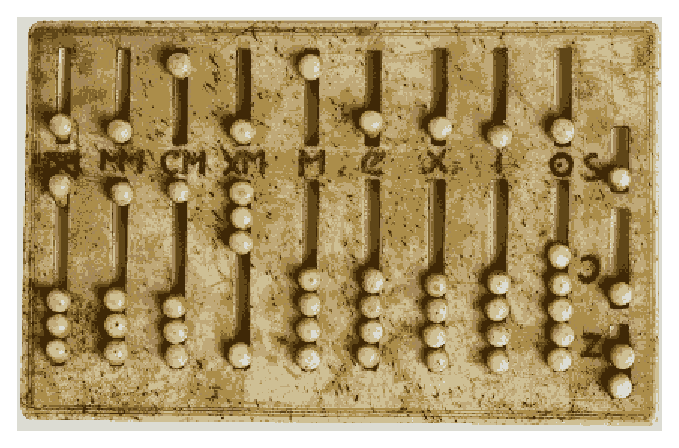
\includegraphics[height=5cm]{Nombres_et_calculs/Images/N2_intro_abaque}
   \caption{Abaque romain en ivoire. INRIA, photo J.-M. Ramès}
\end{figure}

\vfill

\begin{prerequis}[Un peu d'histoire]
   La création des nombres n'a pas été linéaire dans l'histoire : elle s'est faite au gré des croyances, des découvertes, des besoins. Des premiers nombres utilisés pour compter le nombre d'animaux dans un troupeau aux nombres que l'on qualifie de \og complexes \fg{}, la route a été longue. Il a fallu classer ces nombres dans des ensembles, munis d'opérations arithmétiques, ayant des propriétés remarquables. \\
   Concernant les calculs, il y a quelques siècles, compter sur ses doigts était le seul bagage de l'homme. On confiait les multiplications et divisions à quelques calculateurs professionnels que les gens vénéraient comme de véritables sorciers ! Les Babyloniens, les Grecs, les Romains et les Européens utilisent des abaques à jetons au moins jusqu'au Moyen-Âge : des tables sur lesquelles on place des jetons pour caractériser les nombres puis effectuer des calculs. Les pays asiatiques et russes se servent eux de bouliers. Vers 1220, l'italien {\bf Léonardo Fibonacci} rapporte des pays arabes nos chiffres (eux mêmes venus des Indes) et des techniques de calcul plus rapides que les calculs sur abaques. Plus tard, c'est la course à l'invention d'outils et de machines à calculer comme par exemple les réglettes multiplicatrices de {\bf John Neper} en 1617, la Pascaline, première machine à additionner en 1642, la machine analytique de {\bf Charles Babbage} vers 1830, proche du concept de nos ordinateurs.
\end{prerequis}


\cours %%%%%%%%%%%%%%%%%%%%%%%%%%%


\section{Les nombres entiers naturels} %%% 1

   Dès lors que les peuples ont commencé à dénombrer, ils l'ont fait le plus naturellement possible : certains comptaient les bisons, d'autres un nombre de jours\dots{} Les nombres utilisés à cet effet sont les entiers naturels car ce sont ceux que l'on utilise naturellement dans la vie de tous les jours. Il en existe une infinité.

\begin{definition}[$\N$, entiers naturels]
   Un nombre \textbf{entier naturel} est un nombre positif (ou nul) permettant de dénombrer des objets comptant chacun pour un. L'ensemble des entiers naturels est noté $\N$ comme \textit{natural}.
\end{definition}

\medskip

Les entiers naturels permettent de mesurer des collections d'entités discrètes. Ils peuvent se cacher sous des formes \og peu naturelles \fg. 
   
\begin{center}
   \psset{yunit=0.75}
   \begin{pspicture}(5,5)(8,5.5)
      \psframe[linecolor=G1,framearc=0.3](4,4)(8,6)
      \psframe[linecolor=G1,framearc=0.6,linewidth=0.07](4,5.2)(4.8,6)
      \rput(4.4,5.6){\textcolor{G1}{$\N$}}
      \rput(5,5){\textcolor{G1}{$0$}}
      \rput(6,5.5){\textcolor{G1}{$1$}}
      \rput(6,4.5){\textcolor{G1}{$\sqrt{9}$}}
      \rput(7,5.2){\textcolor{G1}{$10^3$}}
      \rput(7.7,4.6){\textcolor{G1}{$\dfrac{6}{3}$}}
   \end{pspicture}
\end{center}

  
\section{Les nombres entiers relatifs} %%% 2

\subsection{Définitions et comparaison} % a
   
\begin{definition}[$\Z$, entiers relatifs]
   Un nombre \textbf{entier relatif} est un entier naturel muni d'un signe positif ou négatif qui indique sa position par rapport à 0. Le nombre sans son signe correspond à sa distance à l'origine. L'ensemble des entiers relatifs est noté $\Z$ comme \textit{Zahl}, nombre en allemand. \smallskip
\end{definition}

\medskip

Tous les entiers naturels sont des entiers relatifs. On note $\N \subset \Z$. 

\begin{center}
   \psset{yunit=0.75}
   \begin{pspicture}(4,3)(9.5,7)
      % N
      \psframe[linecolor=G1,framearc=0.3](4,4)(8,6)
      \psframe[linecolor=G1,framearc=0.6,linewidth=0.07](4,5.2)(4.8,6)
      \rput(4.4,5.6){\textcolor{G1}{$\N$}}
      \rput(5,5){\textcolor{G1}{$0$}}
      \rput(6,5.5){\textcolor{G1}{$1$}}
      \rput(6,4.5){\textcolor{G1}{$\sqrt{9}$}}
      \rput(7,5.2){\textcolor{G1}{$10^3$}}
      \rput(7.7,4.6){\textcolor{G1}{$\dfrac{6}{3}$}}
      % Z
      \psframe[linecolor=B2,framearc=0.2](3,3)(9.5,7)
      \psframe[linecolor=B2,framearc=0.8,linewidth=0.07](3,6.2)(3.8,7)
      \rput(3.4,6.6){\textcolor{B2}{$\Z$}}
      \rput(5,6.5){\textcolor{B2}{$-1$}}
      \rput(8.5,3.5){\textcolor{B2}{$-\sqrt{4}$}}
      \rput(4.1,3.4){\textcolor{B2}{$-37,0$}}
      \rput(8.6,6.4){\textcolor{B2}{$-10\,025$}}
   \end{pspicture}
\end{center}

\begin{definition}[Abscisse et droite graduée]
   Sur une droite graduée, on repère chaque point par un nombre : son {\bf abscisse}.
   \begin{center}
      \begin{pspicture}(-5,-0.4)(5,0.8)
         \psaxes[yAxis=false]{->}(0,0)(-5,0)(5,0)
         \psline[linecolor=B1]{<->}(-5,0.3)(0,0.3)
         \rput(-2.5,0.6){\textcolor{B1}{nombres relatifs négatifs}}
         \psline[linecolor=A1]{<->}(0,0.3)(5,0.3)
         \rput(2.5,0.6){\textcolor{A1}{nombres relatifs positifs}}
      \end{pspicture}
   \end{center}
\end{definition}

\smallskip

\begin{exemple*1}
   L'abscisse de A est $-3$, on note A($-3$) ; l'abscisse de B est 0 et l'abscisse de C est $+4$.
   \begin{center}
      \begin{pspicture}(-5,-0.4)(5,0.5)
         \psaxes[yAxis=false]{->}(0,0)(-5,0)(5,0)
         \rput(-3,0.5){A}
         \rput(0,0.5){B}
         \rput(4,0.5){C}
         \psline[linecolor=B1]{<->}(-3,-0.9)(0,-0.9)
         \rput(-1.5,-1.2){\textcolor{B1}{\small distance à l'origine : 3}}
         \psline[linecolor=A1]{<->}(0,-0.9)(4,-0.9)
         \rput(2,-1.2){\textcolor{A1}{\small distance à l'origine : 4}}
      \end{pspicture}
   \end{center}
\end{exemple*1}

\medskip

\begin{propriete}[Comparaison]
   \begin{itemize}
      \item Deux nombres relatifs négatifs sont rangés dans l'ordre inverse de leur
distance à zéro.
      \item Un nombre relatif négatif est inférieur à un nombre relatif positif.
      \item Deux nombres relatifs positifs sont rangés dans l'ordre de leur distance à zéro. \\ [-8mm]
   \end{itemize}  
\end{propriete}

\begin{exemple*1}
   $-4<-2$ car $4>2$ \qquad ; \quad $-4<2$ car $-4<0$ et $2>0$ \qquad ; \quad $+4>+2$ car $4>2$.
\end{exemple*1}

\smallskip

\begin{remarque}
   les nombres négatifs sont rangés \og dans le sens inverse \fg{} des nombres positifs.
\end{remarque}


\subsection{Opérations avec les entiers relatifs} % b

Dans un calcul, on commence toujours pas effectuer les calculs entre parenthèses, puis les multiplications et divisions, et enfin les additions et soustractions.

\begin{propriete}[Signe]
   \begin{itemize}
      \item Le produit ou le quotient de deux nombres relatifs de même signe est positif.
      \item Le produit ou le quotient de deux nombres relatifs de signes différents est négatif. \smallskip
      \item Dans une fraction, le signe \og $-$ \fg{} se place indifféremment : $\dfrac{-a}{b} =-\dfrac{a}{b} =\dfrac{a}{-b}$ \\ [-6mm]
   \end{itemize}
\end{propriete}

\begin{exemple*1}
      $(-3)\times(-4)= 12$ \qquad $(-4)\times5= -20$ \qquad $25\div(-4)= -6,25$ \qquad $\dfrac{-1}{3} =-\dfrac{1}{3} =\dfrac{1}{-3}$.
\end{exemple*1}


\begin{propriete}[Somme]
   \begin{itemize}
      \item La somme de deux nombres relatifs ayant le même signe s'obtient en ajoutant les distances à 0 et en mettant le même signe que les nombres. 
      \item La somme de deux nombres relatifs n'ayant pas le même signe s'obtient en calculant la différence entre les distances à 0 et en mettant le signe du terme ayant la plus grande distance à 0. \\ [-8mm]
   \end{itemize}
\end{propriete}

\begin{exemple*1}
      $7,3+4=11,3$ \qquad $(-9)+(-5)=-14$ \qquad $(-5)+9= 4$ \qquad $6,2-14= -7,8$.
\end{exemple*1}

\begin{definition}[Opposé]
   L'{\bf opposé} d'un nombre relatif est le  nombre relatif obtenu en changeant son signe. 
\end{definition}

\begin{exemple*1}
   L'opposé de $5 =+5$ est $-5$ ; \qquad  l'opposé de $(-7)$ est $+7 =7$.
\end{exemple*1}

\begin{propriete}[Soustraction]
   Soustraire un nombre revient à ajouter son  opposé : $a-b=a+(-b)$.
\end{propriete}

\begin{exemple*1}
   $-4-(-7)=-4+(+7)=3$ \qquad $10+(-4) =10-4 =6$.
\end{exemple*1}

\ \\

\pagebreak


\section{Les nombres décimaux} %%% 3

\subsection{Défintion} % a
           
\begin{definition}[$\D$, nombres décimaux]
Un nombre \textbf{décimal} est un nombre qui peut s'écrire sous la forme d'une fraction décimale, c'est à dire une fraction dont le dénominateur est une puissance de 10 du type $\dfrac{a}{10^n}$ avec $a\in\Z$. Son ensemble est noté $\D$ comme \textit{décimal}. \smallskip
\end{definition}

\smallskip

   Un nombre décimal possède une quantité quelconque, mais finie de chiffres après la virgule. Contrairement à ce que l'on pourrait croire, les nombres décimaux ont été introduits après les fractions, suite à la découverte des fractions décimales. C'est donc un \textit{cas particulier} des nombres fractionnaires.

\begin{center}  
   \psset{yunit=0.75}
   \begin{pspicture}(2.9,3.3)(11,7)
      % N
      \psframe[linecolor=G1,framearc=0.3](4,4)(8,6)
      \psframe[linecolor=G1,framearc=0.6,linewidth=0.07](4,5.2)(4.8,6)
      \rput(4.4,5.6){\textcolor{G1}{$\N$}}
      \rput(5,5){\textcolor{G1}{$0$}}
      \rput(6,5.5){\textcolor{G1}{$1$}}
      \rput(6,4.5){\textcolor{G1}{$\sqrt{9}$}}
      \rput(7,5.2){\textcolor{G1}{$10^3$}}
      \rput(7.7,4.6){\textcolor{G1}{$\dfrac{6}{3}$}}
      % Z
      \psframe[linecolor=B2,framearc=0.2](3,3)(9.5,7)
      \psframe[linecolor=B2,framearc=0.8,linewidth=0.07](3,6.2)(3.8,7)
      \rput(3.4,6.6){\textcolor{B2}{$\Z$}}
      \rput(5,6.5){\textcolor{B2}{$-1$}}
      \rput(8.5,3.5){\textcolor{B2}{$-\sqrt{4}$}}
      \rput(4.1,3.4){\textcolor{B2}{$-37,0$}}
      \rput(8.6,6.4){\textcolor{B2}{$-10\,025$}}
      % D
      \psframe[linecolor=A1,framearc=0.1](2,2)(11,8)
      \psframe[linecolor=A1,framearc=1,linewidth=0.07](2,7.2)(2.8,8)
      \rput(2.4,7.6){\textcolor{A1}{$\D$}}
      \rput(6.5,7.5){\textcolor{A1}{$0,008$}}
      \rput(4.5,2.5){\textcolor{A1}{$-1,2$}}
      \rput(10.1,6.2){\textcolor{A1}{$\dfrac{3}{25}$}}
      \rput(10.4,3.2){\textcolor{A1}{$\dfrac{1}{10^6}$}}
   \end{pspicture}
\end{center}
      

\subsection{Reconnaître un nombre décimal} % b

\begin{methode*2*2}[Déterminer si un nombre est décimal]
Pour reconnaître qu'un nombre exprimé sous forme de fraction est un nombre décimal, on peut effectuer les étapes suivantes :
\begin{itemize}
   \item mettre le nombre sous forme de fraction irréductible ;
   \item si le dénominateur est de la forme $2^n\times5^p$ (où $n$ et $p$ sont des entiers naturels), c'est à dire si le dénominateur ne comporte que des puissances de 2 et de 5, alors ce nombre est décimal ; sinon, ce nombre n'est pas décimal. 
\end{itemize}
\exercice
   $\dfrac{21}{140}$ est-il un décimal ?
\correction
   \begin{itemize}
      \item On commence par mettre la fraction sous la forme d'une fraction irréductible : \\ [1mm] 
      $\dfrac{21}{140} =\dfrac{3\times\cancel7}{20\times\cancel7} =\dfrac{3}{20}$. \\ [-1mm]
      \item Puis on décompose le dénominateur en produit de facteurs premiers : $\dfrac{3}{20} =\dfrac{3}{2^2\times5}$. \\ [1mm] 
      Le dénominateur ne comporte que des puissances de 2 et de 5, donc il est décimal. \\
      Son écriture décimale est 0,15.
   \end{itemize}
\exercice
   $\dfrac{3}{140}$ est-il décimal ?
\correction
   \begin{itemize}
      \item La fraction est déjà sous forme irréductible.
      \item On décompose le dénominateur en produit de facteurs premiers : $\dfrac{3}{140} = \dfrac{3}{2^2\times5\times7}$ \\ [1mm]
      Le dénominateur comporte le nombre 7, donc il n'est pas décimal.
   \end{itemize}
\end{methode*2*2}


\pagebreak


\section{Les nombres rationnels} %%% 4

\subsection{Définition} % a

   De tout temps, l'homme a souhaité partager des quantités, prémisse de ce qu'on appellera bien plus tard les fractions. Ces nombres que l'on \og coupait \fg{} étaient appelés les \textit{nombres rompus}.
   
\begin{definition}[$\Q$, nombres rationnels]
   Les \textbf{nombres rationnels} sont les nombres pouvant s'écrire sous la forme d'une fraction $\dfrac{p}{q}$ où $p$ et $q$ sont des entiers relatifs (non nul pour $q$). Cet ensemble est noté $\Q$ comme \textit{quotient}. 
\end{definition}

\begin{center}  
   \psset{yunit=0.75}
   \begin{pspicture}(2,1.5)(12.5,9)
      % N
      \psframe[linecolor=G1,framearc=0.3](4,4)(8,6)
      \psframe[linecolor=G1,framearc=0.6,linewidth=0.07](4,5.2)(4.8,6)
      \rput(4.4,5.6){\textcolor{G1}{$\N$}}
      \rput(5,5){\textcolor{G1}{$0$}}
      \rput(6,5.5){\textcolor{G1}{$1$}}
      \rput(6,4.5){\textcolor{G1}{$\sqrt{9}$}}
      \rput(7,5.2){\textcolor{G1}{$10^3$}}
      \rput(7.7,4.6){\textcolor{G1}{$\dfrac{6}{3}$}}
      % Z
      \psframe[linecolor=B2,framearc=0.2](3,3)(9.5,7)
      \psframe[linecolor=B2,framearc=0.8,linewidth=0.07](3,6.2)(3.8,7)
      \rput(3.4,6.6){\textcolor{B2}{$\Z$}}
      \rput(5,6.5){\textcolor{B2}{$-1$}}
      \rput(8.5,3.5){\textcolor{B2}{$-\sqrt{4}$}}
      \rput(4.1,3.4){\textcolor{B2}{$-37,0$}}
      \rput(8.6,6.4){\textcolor{B2}{$-10\,025$}}
      % D
      \psframe[linecolor=A1,framearc=0.1](2,2)(11,8)
      \psframe[linecolor=A1,framearc=1,linewidth=0.07](2,7.2)(2.8,8)
      \rput(2.4,7.6){\textcolor{A1}{$\D$}}
      \rput(6.5,7.5){\textcolor{A1}{$0,008$}}
      \rput(4.5,2.5){\textcolor{A1}{$-1,2$}}
      \rput(10.1,6.2){\textcolor{A1}{$\dfrac{3}{25}$}}
      \rput(10.4,3.2){\textcolor{A1}{$\dfrac{1}{10^6}$}}
      %Q
      \psframe[linecolor=PartieStatistique,framearc=0.1](1,1)(12.5,9)
      \psframe[linecolor=PartieStatistique,framearc=1,linewidth=0.07](1,8.2)(1.8,9)
      \rput(1.4,8.6){\textcolor{PartieStatistique}{$\Q$}}
      \rput(3,8.5){\textcolor{PartieStatistique}{$0,33\underline{3}$}}
      \rput(11.6,5.2){\textcolor{PartieStatistique}{$-\dfrac{13}{19}$}}
      \rput(11.5,2){\textcolor{PartieStatistique}{$\dfrac{1}{6}$}}
      \rput(4,1.5){\textcolor{PartieStatistique}{$\sqrt{\frac{4}{9}}$}}
   \end{pspicture}
\end{center}


\subsection{Calculer avec des fractions} % b

\begin{propriete}[Multiplication ou division par un nombre]
   On ne change pas la valeur d'une fraction en multipliant ou en divisant le numérateur et le dénominateur par un même nombre relatif non nul.
   $${a\times k\over b\times k}={a\over b} \qquad ; \qquad {a\div k\over b\div k}={a\over b}$$
\end{propriete}

\begin{exemple*1}   
   $\displaystyle{{5\over13}={5\times3\over13\times3}={15\over39}}$ \hskip2cm $\displaystyle{{15\over39}={15\div3\over39\div3}={5\over13}}$
\end{exemple*1}
\begin{remarque}
   on peut utiliser cette propriété pour simplifier une fraction : $\displaystyle{{18\over27}={2\times\cancel9\over3\times\cancel9}={2\over3}}$.
\end{remarque}


\begin{propriete}[Produit]
   On obtient le produit de deux nombres fractionnaires en multipliant les numérateurs entre eux et les dénominateurs entre eux et en formant une nouvelle fraction avec ces produits.
   $${a\over b}\times{c\over d}={ac\over bd}$$
\end{propriete}

\begin{exemple*1}
   $\displaystyle{{4\over-3}\times{-7\over -5} ={4\times(-7)\over-3\times(-5)} ={-28\over15} =-{28\over15}}$.
\end{exemple*1}


\begin{definition}[Inverse]
   L'\textbf{inverse} d'un nombre $x$ non nul est le nombre $x^{-1} =\dfrac1x$ par lequel on le multiplie pour obtenir $1$.
   $$x\times x^{-1} =x^{-1}\times x =x\times\dfrac1x =\dfrac1x\times x =1$$
\end{definition}

\begin{exemple*1}
   L'inverse de 10 est $\dfrac{1}{10} =1\div10 =0,1$. \\
   L'inverse de 3 est $\dfrac13 =1\div3=0,\overline{3} =0,333\dots$. Le résultat n'est pas un nombre décimal.
\end{exemple*1}


\begin{propriete}[Division]
   Diviser par un nombre revient à multiplier par son inverse.
  $$\frac{a}b : c=\frac{a}b\times\frac1c =\frac{a}{bc} \qquad ; \qquad \frac{a}b : \frac{c}d =\frac{a}b\times\frac{d}c =\frac{ad}{bc}$$
\end{propriete}

\begin{exemple*1}
   $\displaystyle{{5\over3}\div{3\over-7} ={5\over3}\times{-7\over 3} ={5\times(-7)\over{3\times3}} ={-35\over 9} =-{35\over 9}}$.
\end{exemple*1}


\begin{propriete}[Addition de fractions de même dénominateur]
   Pour additionner [resp. soustraire] deux fractions ayant le même dénominateur, on ajoute [resp. soustrait] les numérateurs et on garde le même dénominateur :
   $${a\over c}+{b\over c}={a+b\over c} \qquad \text{et} \qquad {a\over c}-{b\over c}={a-b\over c}$$
\end{propriete}

\begin{exemple*1}
   $\displaystyle{{-4\over7}-{-12\over 7}={-4-(-12)\over 7}={-4+12\over 7}={8\over 7}}$.
\end{exemple*1}

\smallskip

\begin{propriete}[Addition de fractions de  dénominateurs différents]
   Pour additionner ou soustraire deux fractions ayant des dénominateurs différents, on transforme l'écriture des fractions pour qu'elles aient le même dénominateur.
\end{propriete} 

\begin{exemple*1}
   $\displaystyle{{-4\over3\mathstrut}+{5\over2} ={-4\times2\over3\times 2}+{5\times3\over2\times3} = {-8\over6}+{15\over6} ={-8+15\over6}={7\over6}}$.
\end{exemple*1}

\ \\


\pagebreak


\section{Les nombres réels} %%% 5

   Aux alentours du $\cRm{5}$\up{e} siècle av. J.-C., des mathématiciens grecs démontrent que les longueurs de la diagonale du carré et de son côté sont incommensurables. Nous disons aujourd'hui que ce rapport, de longueur $\sqrt{2}$, est {\bf irrationnel}, c'est-à-dire qu'il n'est pas égal à une fraction. Ceci met en évidence que l'ensemble $\Q$ ne peut suffire pour représenter toutes les grandeurs mesurables et qu'il faut construire un ensemble plus grand.
   
\begin{definition}[$\R$, nombres réels]
   Un nombre \textbf{réel} est un nombre qui peut être représenté par une partie entière et une liste finie ou infinie de décimales. Son ensemble est noté $\R$ comme \textit{réal}. \smallskip
\end{definition}

\medskip

On trouve dans cet ensemble et pas ailleurs, par exemple, les nombres $\pi$, $\sqrt2$, $\sqrt[3]{5}$, $e$\dots \\
On représente cet ensemble par une droite graduée appelée droite numérique. Tout point de cette droite a pour abscisse un nombre réel et tout nombre réel est l'abscisse d'un point de cette droite. On a alors :
$$\N \subset \Z \subset \D \subset \Q \subset \R$$

\smallskip

\begin{definition}[Intervalle]
   L’ensemble des nombres réels compris entre $a$ et $b$ (inclus) est appelé intervalle et se note $[\,a\,;\,b\,]$. $a$ et $b$ sont les bornes de l’intervalle.
\end{definition}

\medskip

On peut définir plusieurs types d'intervalle :
\begin{center}
   {\hautab{1.25}
   \begin{ltableau}{0.7\linewidth}{3}
      \hline
      Inégalité & Notation & Représentation \\
      \hline
      $a\leq x\leq b$ & $x\in[\,a\,;\,b\,]$ & \psline{->}(-1,0.15)(1,0.15) \psline[linecolor=red]{[-]}(-0.5,0.15)(0.5,0.15) \rput(-0.5,-0.05){\red\scriptsize $a$} \rput(0.5,-0.05){\red\scriptsize b} \\
      \hline
      $a< x\leq b$ & $x\in\,]\,a\,;\,b\,]$ & \psline{->}(-1,0.15)(1,0.15) \psline[linecolor=red]{]-]}(-0.5,0.15)(0.5,0.15) \rput(-0.5,-0.05){\red\scriptsize $a$} \rput(0.5,-0.05){\red\scriptsize b} \\
      \hline
      $a\leq x< b$ & $x\in[\,a\,;\,b\,[$ & \psline{->}(-1,0.15)(1,0.15) \psline[linecolor=red]{[-[}(-0.5,0.15)(0.5,0.15) \rput(-0.5,-0.05){\red\scriptsize $a$} \rput(0.5,-0.05){\red\scriptsize b} \\
      \hline
      $a< x< b$ & $x\in\,]\,a\,;\,b\,[$ & \psline{->}(-1,0.15)(1,0.15) \psline[linecolor=red]{]-[}(-0.5,0.15)(0.5,0.15) \rput(-0.5,-0.05){\red\scriptsize $a$} \rput(0.5,-0.05){\red\scriptsize b} \\
      \hline
      $x\geq a$ & $x\in[\,a\,;\,+\infty\,[$ & \psline{->}(-1,0.15)(1,0.15) \psline[linecolor=red]{[->}(-0.5,0.15)(1,0.15) \rput(-0.5,-0.05){\red\scriptsize $a$} \\
      \hline
      $x> a$ & $x\in\,]\,a\,;\,+\infty\,[$ & \psline{->}(-1,0.15)(1,0.15) \psline[linecolor=red]{]->}(-0.5,0.15)(1,0.15) \rput(-0.5,-0.05){\red\scriptsize $a$} \\
      \hline
      $x\leq b$ & $x\in\,]\,-\infty\,;\,b\,]$ & \psline{->}(-1,0.15)(1,0.15) \psline[linecolor=red]{-]}(-1,0.15)(0.5,0.15) \rput(0.5,-0.05){\red\scriptsize $b$} \\
      \hline
      $x< b$ & $x\in\,]\,-\infty\,;\,b\,[$ & \psline{->}(-1,0.15)(1,0.15) \psline[linecolor=red]{-[}(-1,0.15)(0.5,0.15) \rput(0.5,-0.05){\red\scriptsize $b$} \\
      \hline
   \end{ltableau}}
\end{center}

Les signes $-\infty$ et $+\infty$ se lisent \og moins l'infini \fg{} et \og plus l'infini \fg. L'ensemble $\R$ s'écrit aussi $]-\infty\,;\,+\infty\,[$.

\smallskip

\begin{definition}[Valeur absolue et distance]
   On considère une droite graduée d'origine $O$ et des points $A$ et $B$ d'abscisses $a$ et $b$.
   \begin{itemize}
      \item La valeur absolue de $a$, notée $|a|$ est le nombre égal à la distance $OA$.
      \item On appelle distance entre les réels $a$ et $b$ la distance $AB$, notée $|a-b|$. \smallskip
   \end{itemize}
\end{definition}

\smallskip

\begin{exemple*1}
   \begin{center}
      \begin{pspicture}(-5.5,-0.5)(5,0)
         \psline{->}(-5,0)(5,0)
         \rput(-3,0.4){$A$}
         \rput(-3,-0.4){\small $-3$}
         \rput(0,0.4){$O$}
         \rput(0,-0.4){0}
         \rput(4,0.4){$B$}
         \rput(4,-0.4){\small $4$}
         \multido{\n=-4+1}{9}{\rput(\n,0){|}}
         \psline[linecolor=B1]{<->}(-3,-0.7)(0,-0.7)
         \rput(-1.5,-1){\textcolor{B1}{\small $|a| =3$}}
         \psline[linecolor=A1]{<->}(0,-0.7)(4,-0.7)
         \rput(2,-1){\textcolor{A1}{\small $|b| =4$}}
         \psline[linecolor=blue]{<->}(-3,-1.3)(4,-1.3)
         \rput(0.5,-1.6){\textcolor{blue}{\small $|a-b| =7$}}
      \end{pspicture}
   \end{center}
\end{exemple*1}



%%%%%%%%%%%%%%%%%%%%%%%%%
%%%%%%%%%%%%%%%%%%%%%%%%%
\activites


\begin{activite}[Groupement 3 - Exercice 3 - Partie C : calculs et fractions]
   \ \\ [-16mm]
   \begin{QCM}
      Dans la perspective d’offrir des bouquets de fleurs pour la fête de l’école, l’enseignante souhaite planter des graines dans le potager. Dans la classe il y a 26 élèves et chaque élève reçoit 20 graines à semer. \\
On a reporté ci-dessous ce que l’on peut  lire sur le paquet de graines choisi.
      \begin{center}
         \fbox{\begin{minipage}{6cm}
            \ \\
            Taux de germination des graines : 90\,\% \\ [1mm]
            Prix du paquet de graines : 4,53 \euro. \\ [1mm]
            Ce paquet contient 50 graines. \\ [1mm]
            Période de semis : d’avril à juin. \\ [1mm]
            Hauteur adulte : 50 cm. \\
         \end{minipage}
      }
      \end{center}
      On rappelle que le taux de germination d’un paquet de graines indique le pourcentage de graines qui devraient germer et donc produire une fleur.
      \begin{enumerate}
         \item Combien de fleurs un élève peut-il espérer voir pousser ? 
         \item Quel sera le budget à prévoir pour l’achat des graines ?
         \item En plus des graines, des bulbes de tulipes et de jonquilles sont plantés.
            \begin{enumerate}
               \item L’enseignante en plante sur un sixième du potager puis un peu plus loin sur un huitième de ce même potager. \\
                  Un élève affirme que les bulbes représentent plus de 25\,\% du potager. À-t-il raison ? Justifier votre réponse.
              \item Elle met dans un panier 30 bulbes de jonquilles et des bulbes de tulipes. La proportion de bulbes de jonquilles dans le panier est de $\dfrac56$. \\ [1mm]
                 Calculer le nombre de bulbes de tulipes dans ce panier. \medskip
           \end{enumerate}
     \end{enumerate}
   \end{QCM}
   
   \bigskip
     
   \textcolor{G1}{
   {\bf Exemple de corrigé.} \smallskip
      \begin{enumerate}
         \item Un élève reçoit 20 graines, dont le taux de germination est de 90\,\%. \\ [1mm]
            Cela fait : $\dfrac{90}{100}\times20\text{ graines} =18\text{ graines}$. \\ [1mm]
            \uline{Chaque élève peut espérer voir pousser 18 graines}.
         \item Pour les 26 élèves, il faut acheter $26\times20\text{ graines} =520\text{ graines}$. \\
            Un paquet contenant 50 graines, il faut donc acheter 11 paquets ($11\times50\text{ graines} =550\text{ graines}$). \\
            Un paquet de graines coûte 4,53 \euro, ce qui fait un budget de $11\times4,53\text{ \euro} =49,83\text{ \euro}$. \\
            \uline{Le budget à prévoir pour l'achat des graines est de 49,83 \euro}. \smallskip
         \item
            \begin{enumerate}
               \item $\dfrac16+\dfrac18 =\dfrac8{48}+\dfrac6{48} =\dfrac{14}{48} =\dfrac{7}{24}$. \\ [1mm]
                  Or, $25\,\% =\dfrac14 =\dfrac{6}{24}$ qui est plus petit que $\dfrac7{24}$. \\ [1mm]
                  \uline{Les bulbes représentent plus de 25\,\% du potager, l'élève a raison}. \smallskip     
               \item Un proportion de jonquilles de $\dfrac56$ signifie que, pour 5 bulbes jonquilles, on a 1 bulbe de tulipe. \\ [1mm]
                 Par conséquent, si on a 30 bulbes jonquilles (donc 6 fois plus), alors on a 6 bulbes de tulipes. \\
                 \uline{Il y a 6 bulbes de tulipes dans le panier}. \\
           \end{enumerate}
      \end{enumerate}
   }
\end{activite}

\pagebreak


\begin{activite}[Groupement 3 - Exercice 1 - Questions 4 à 6 : fractions]
   \ \\ [-16mm]
   \begin{QCM}
      Pour chacune des questions, une seule des quatre réponses proposées est exacte. Donner la bonne réponse en la justifiant. \\
      {\it Une réponse erronée n’enlève pas de point. Une réponse non justifiée ne rapporte pas de point.}
      \begin{center}
         \hautab{1.5}{
         \begin{tabular}{|C{0.1}p{4cm}|*{4}{C{2}|}}
            \hline
            & \bf Questions : & \bf A & \bf B & \bf C & \bf D \\
            \hline
            1.
            & \rule{0mm}{6mm} $\dfrac{4}{25}$ est \dots
            & un nombre réel mais n’est pas un nombre rationnel.
            & un nombre rationnel mais n’est pas un nombre décimal.
            & un nombre décimal mais n’est pas un nombre entier.
            & un nombre entier. \\
            \hline
            2.  
            & \rule[-4.5mm]{0mm}{11mm} Le quart de $\dfrac4{12}$ est\dots
            & $\dfrac13$
            & $\dfrac43$
            & $\dfrac{16}{48}$
            & $\dfrac{4}{48}$ \\
           \hline
            3.
            & \rule[-4.5mm]{0mm}{11mm} $\dfrac23\times5+5\times\dfrac13$ est égale à
            & 5
            & $\dfrac{20}{9}$
            & $\dfrac{15}{15}$
            & $\dfrac{20}{90}$ \\
            \hline
         \end{tabular}}
      \end{center} \bigskip
   \end{QCM}

   \bigskip
   
   \textcolor{G1}{
   {\bf Exemple de corrigé.} \smallskip
      \begin{enumerate}      
         \item $\dfrac4{25} =\dfrac{16}{100} =0,16$ donc, cette fraction est un nombre décimal mais n'est pas un entier. \hfill \uline{La réponse est C}. \medskip 
         \item $\dfrac14\times\dfrac4{12} =\dfrac4{48}$. \hfill \uline{La réponse est D}. \medskip 
         \item $\dfrac23\times5+5\times\dfrac13 =\dfrac{10}{3}+\dfrac53 =\dfrac{15}{3} =5$. \hfill \uline{La réponse est A}.
     \end{enumerate}} 
\end{activite}


%%%%%%%%%%%%%%%%%%%%%%%%%%%%%%
%%%%%%%%%%%%%%%%%%%%%%%%%%%%%%
\exercicesbase

\begin{center}
   {\cursive Maîtriser les bases avec} \href{http://mathenpoche.sesamath.net}{
\includegraphics[width=3cm]{Nombres_et_calculs/Images/mathenpoche}} \\
   \bigskip
   {\hautab{0.85}
   \cursive
      \begin{Ltableau}{0.775\linewidth}{4}{C{1}|C{1}|p{7cm}|p{2.3cm}}
         \hline
         Classe & \texttt{N\degre} & Thème & Dans le cours \\
         \hline
         \textcolor{orange}{\bf 6\up{e}} & \texttt{N1} & Nombres entiers et décimaux & 1. et 3. \\
         & \texttt{N3} & Opérations & 1. à 3. \\   
         & \texttt{N5} & Fractions, écritures fractionnaires & 4. \\
         \hline
         \textcolor{cyan}{\bf 5\up{e}} & \texttt{A1} & Nombres décimaux & 3. \\
         & \texttt{A2} & Nombres relatifs & 2. \\
         & \texttt{A3} & Nombres rationnels & 4. \\
         \hline
         \textcolor{violet}{\bf 4\up{e}} & \texttt{A1} & Nombres décimaux & 3. \\
         & \texttt{A2} & Nombres relatifs & 2. \\
         & \texttt{A3} & Nombres rationnels & 4. \\
         \hline
         \textcolor{green}{\bf 3\up{e}} & \texttt{A3} & Nombres rationnels & 4. \\
         \hline
         \textcolor{red}{\bf 2\up{nde}} & \texttt{N3} & Intervalles et inégalités & 5. \\
         \hline
      \end{Ltableau}
   }
\end{center}


\bigskip


\begin{exercice}[Meli-mélo de calculs] %%% 1
   Effectuer les calculs suivants à la main.
   \begin{multicols}{3}
      \begin{bigenumerate}
         \item $A =|123,45|$ \\
         \item $B =123,2+12,32+1,232$ \\
         \item $C =(-2)\times(-8)$ \\
         \item $D =\dfrac{2}{3}\times\dfrac{4}{7}$
         \item $E =-5\times\dfrac{-2}{3}$ \\
         \item $F=\dfrac{3}{4}+\dfrac{7}{6}$ \\
         \item $G =3,728\times15,12$ \\
         \item $H =(+2)+(-13)$
         \item $I =13\,235-788$ \\
         \item $\,J =|-12|$ \\
         \item $\,K =(-5)+(-14)$ \\
         \item $\,L =\left|-\dfrac14\right|$
      \end{bigenumerate}
   \end{multicols}
\end{exercice}
 
\begin{corrige}
\ \\
   \vspace*{-9mm}
   \begin{multicols}{2}
      \begin{bigenumerate}
         \item $A =|123,45| ={\blue 123,45}$. \\ [3mm]
         \item $B =123,2+12,32+1,232 ={\blue 136,752}$. \\ [3mm]
         \item $C =(-2)\times(-8) ={\blue 16}$. \\ [3mm]
         \item $D =\dfrac{2}{3}\times\dfrac{4}{7} = {\blue \dfrac{8}{21}}$. \\ [3mm]
         \item $E =-5\times\dfrac{-2}{3} ={\blue \dfrac{10}{3}}$. \\ [3mm]
         \item $F=\dfrac{3}{4}+\dfrac{7}{6} =\dfrac{9}{12}+\dfrac{14}{12} ={\blue \dfrac{23}{12}}$. \\ [3mm]   
         \item $G =3,728\times15,12 ={\blue 56,36736}$. \\ [3mm]
         \item $H =(+2)+(-13) ={\blue -11}$. \\ [3mm]
         \item $I =13\,235-788 ={\blue 12\,447}$. \\ [3mm]
         \item $J =|-12| ={\blue 12}$. \\ [3mm]
         \item $K =(-5)+(-14) ={\blue -19}$. \\ [3mm]
         \item $L =\left|-\dfrac14\right| ={\blue \dfrac14}$.
      \end{bigenumerate}
   \end{multicols}
\end{corrige}


\bigskip


\begin{exercice}[Multiplication par les aires] %%% 2
   La technique \og classique \fg{} de la multiplication peut être modélisée par des aires. \\
   Par exemple, pour $5\times 23$, on modélise ici la situation par un schéma qui n'est pas à l'échelle : \\ [2mm]
   \begin{minipage}{7cm}
      \begin{pspicture}(-0.5,0)(5,2.5)
         \psframe[fillstyle=solid,fillcolor=gray!75](0,0)(3.5,2)
         \psframe[fillstyle=solid,fillcolor=gray!25](3.5,0)(5,2)
         \rput(1.75,1.25){$5\times20$}
         \rput(1.75,0.75){$=100$}
         \rput(4.25,1.25){$5\times3$}
         \rput(4.25,0.75){$ =15$}
         \rput(-0.3,1){5}
         \rput(1.75,2.3){20}
         \rput(4.25,2.3){3}
      \end{pspicture}
   \end{minipage}   
   \begin{minipage}{5.5cm}
      Écriture en ligne : \\
      \begin{tabular}[t]{p{9mm}p{3cm}}
         $5\times23$ & $=5\times(20+3)$ \\
         & $=5\times20+ 5\times3$ \\
         & $=100+15$ \\
         & $=115$ \\
      \end{tabular}
   \end{minipage}
   \begin{minipage}{5cm}
      Écriture en colonnes : \\
      \hspace*{5mm}
      {\hautab{0.9}
      \begin{tabular}[t]{*{4}{C{0}}}
         & & 5 \\
         $\times$ & 2 & 3 \\
         \hline
         & 1 & 5 \\
         1 & 0 & 0 \\
         \hline
         1 & 1 & 5 \\
      \end{tabular}}
   \end{minipage} \\ [3mm]
   \begin{enumerate}
      \item Quelle propriété de la multiplication ces trois représentations mettent-elles en valeur ?
      \item Représenter sous forme d'aires, d'écriture en ligne et en colonnes les deux opérations suivantes :
      \begin{colenumerate}{2}
         \item $43\times69$
         \item $234\times75$
      \end{colenumerate}
   \end{enumerate}
\end{exercice}

\begin{corrige}
\ \\ [-5mm]
  \begin{enumerate}
      \item Il s'agit de la {\blue distributivité de la multiplication par rapport à l'addition}.
      \item
         \begin{enumerate}
            \item {\blue $43\times69 =2\,967$}. \\
               \begin{minipage}{6.5cm}
                  \begin{pspicture}(0,-2)(5,2.8)
                     \psframe[fillstyle=solid,fillcolor=gray!80](0,0)(3.5,2)
                     \psframe[fillstyle=solid,fillcolor=gray!60](3.5,0)(5,2)
                     \psframe[fillstyle=solid,fillcolor=gray!40](0,-1)(3.5,0)
                     \psframe[fillstyle=solid,fillcolor=gray!20](3.5,-1)(5,0)
                     \rput(1.75,1){\footnotesize \parbox{12mm}{$60\times40\\=2\,400$}}
                     \rput(4.25,1){\footnotesize \parbox{8mm}{$60\times3\\=180$}}
                     \rput(1.75,-0.5){\footnotesize \parbox{8mm}{$9\times40\\=360$}}
                     \rput(4.25,-0.5){\footnotesize \parbox{7mm}{$9\times3\\=27$}}
                     \rput(-0.3,1){60}
                     \rput(-0.3,-0.5){9}
                     \rput(1.75,2.3){40}
                     \rput(4.25,2.3){3}
                     \rput(5.5,1){\footnotesize 2\,580}
                     \rput(5.4,-0.5){\footnotesize 387}
                  \end{pspicture}
               \end{minipage}   
               \begin{minipage}{7.4cm}
                  Écriture en lignes : \\ [2mm]
                  {\hautab{1.25}
                  \begin{tabular}[t]{p{7mm}p{5cm}}
                     $43\times69\!\!\!\!\!\!$ & $=(40+3)\times(60+9)$ \\
                     & $=40\times60+40\times9+3\times60+3\times9$ \\
                     & $=2\,400+360+180+27$ \\
                     & $=2\,967$ \\
                  \end{tabular}}
               \end{minipage}
               \begin{minipage}{1.7cm}
                  Écriture en colonnes : \\ [2mm]
                     \begin{tabular}[t]{*{5}{C{0}}}
                        & & 4 & 3 \\
                        $\times$ & & 6 & 9 \\
                        \hline
                        & 3 & 8 & 7 \\
                        2 & 5 & 8 & 0 \\
                        \hline
                        2 & 9 & 6 & 7 \\
                     \end{tabular}
               \end{minipage}
      \item 
      {\blue $234\times75 =17\,750$}. \\
         \begin{minipage}{7.3cm}
            \begin{pspicture}(0,-2.5)(7,2.8)
               \psframe[fillstyle=solid,fillcolor=gray!80](0,0)(3.5,2)
               \psframe[fillstyle=solid,fillcolor=gray!65](3.5,0)(5,2)
               \psframe[fillstyle=solid,fillcolor=gray!50](0,-1)(3.5,0)
               \psframe[fillstyle=solid,fillcolor=gray!35](3.5,-1)(5,0)
               \psframe[fillstyle=solid,fillcolor=gray!20](5,0)(6,2)
               \psframe[fillstyle=solid,fillcolor=gray!5](5,0)(6,-1)
               \rput(1.75,1){\footnotesize \parbox{12mm}{$70\times200\\=14\,000$}}
               \rput(4.25,1){\footnotesize \parbox{10mm}{$70\times30\\=2\,100$}}
               \rput(1.75,-0.5){\footnotesize \parbox{10mm}{$5\times200\\=1\,000$}}
               \rput(4.25,-0.5){\footnotesize \parbox{8mm}{$5\times30\\=150$}}
               \rput(5.5,1){\footnotesize \parbox{8mm}{$70\times4\\=280$}}
               \rput(5.5,-0.5){\footnotesize \parbox{7mm}{$5\times4\\=20$}}
               \rput(-0.3,1){70}
               \rput(-0.3,-0.5){5}
               \rput(1.75,2.3){200}
               \rput(4.25,2.3){30}
               \rput(5.5,2.3){4}
               \rput(6.6,1){\footnotesize 16\,380}
               \rput(6.55,-0.5){\footnotesize 1\,170}
            \end{pspicture}
         \end{minipage}   
         \begin{minipage}{6.3cm}
            Écriture en lignes : \\ [2mm]
            $234\times75$ \\ [1mm]
            $=(200+30+4)\times(70+5)$ \\ [1mm]
            $=200\times70+200\times5+30\times70$ \\ [-1mm]
            \hspace*{2mm} $+30\times5+4\times70+4\times5$ \\ [1mm]
            $=14\,000+1\,000+2\,100+150+280+20$ \\ [1mm]
            $=17\,550$ \\ [1mm]
         \end{minipage}
         \begin{minipage}{2cm}
            Écriture en colonnes : \\ [2mm]
               \begin{tabular}[t]{*{5}{C{0}}}
                  & & 2 & 3 & 4 \\
                  $\times$ & & & 7 & 5 \\
                  \hline
                  & 1 & 1 & 7 & 0 \\
                  1 & 6 & 3 & 8 & 0 \\
                  \hline
                  1 & 7 & 7 & 5 & 0 \\ [1mm]
               \end{tabular}
            \end{minipage} 
      \end{enumerate}
   \end{enumerate}
\end{corrige}


\bigskip



\begin{exercice}[Le bon intervalle] %%% 3
\ \\ [-14mm]
   \begin{multicols}{2}
      \begin{enumerate}
         \item Pour chacune des droites graduées, donner l'inégalité correspondant à la partie colorée puis l'intervalle correspondant.
            \begin{enumerate}
               \item {\psset{unit=0.7}
                        \begin{pspicture}(-5.5,-0.2)(5,1)
                           \psline{->}(-5,0)(5,0)
                           \multido{\n=-4+1}{8}{\rput(\n,0){|}}
                           \rput(0,-0.4){0}
                           \rput(1,-0.4){1}
                           \psline[linewidth=0.6mm,linecolor=B1]{[-]}(-3,0)(4,0)
                        \end{pspicture}}
               \item {\psset{unit=0.7}
                        \begin{pspicture}(-5.5,-0.2)(5,1)
                           \psline{->}(-5,0)(5,0)
                           \multido{\n=-4+1}{8}{\rput(\n,0){|}}
                           \rput(0,-0.4){0}
                           \rput(1,-0.4){1}
                           \psline[linewidth=0.6mm,linecolor=B1]{-]}(-5,0)(3,0)
                        \end{pspicture}}
               \item {\psset{unit=0.7}
                        \begin{pspicture}(-5.5,-0.2)(5,1)
                           \psline{->}(-5,0)(5,0)
                           \multido{\n=-4+1}{8}{\rput(\n,0){|}}
                           \rput(0,-0.4){0}
                           \rput(1,-0.4){1}
                           \psline[linewidth=0.6mm,linecolor=B1]{]-}(-1,0)(5,0)
                        \end{pspicture}}
               \item {\psset{unit=0.7}
                        \begin{pspicture}(-5.5,-0.2)(5,1)
                           \psline{->}(-5,0)(5,0)
                           \multido{\n=-4+1}{8}{\rput(\n,0){|}}
                           \rput(0,-0.4){0}
                           \rput(1,-0.4){1}
                           \psline[linewidth=0.6mm,linecolor=B1]{]-[}(-1.5,0)(1.5,0)
                        \end{pspicture}}
            \end{enumerate}
         \item Pour chaque inégalité, représenter la solution sur une droite graduée puis donner l'intervalle correspondant. \medskip
            \begin{enumerate}
               \item $-2,5\leq x<1$. \\
               \item $x\geq2$. \\
               \item $-4,2<x\leq2,3$. \\
               \item $x<3$.
            \end{enumerate}
      \end{enumerate}
   \end{multicols}
\end{exercice}

\begin{corrige}
\ \\ [-10mm]
   \begin{minipage}{6.5cm}
      \begin{enumerate}
         \item 
            \begin{enumerate}
               \item {\blue $x\in\,[-3\,;\,4\,]$} et {\blue $-3\leq x\leq 4$}.
               \item {\blue $x\in\,]-\infty\,;\,3\,]$} et {\blue $x\leq 3$}.
               \item {\blue $x\in\,]-1\,;\,+\infty\,[$} et {\blue $x>-1$}.
               \item {\blue $x\in\,]-1,5\,;\,1,5\,[$} et {\blue $-1,5< x<1,5$}.
            \end{enumerate}
      \end{enumerate}
   \end{minipage}
   \begin{minipage}{9.5cm}
      \begin{enumerate}     
      \setcounter{enumi}{1}
         \item 
            \begin{enumerate}
            \setcounter{enumi}{1}
               \item {\psset{unit=0.6}
                        \begin{pspicture}(-4.7,-0.2)(5,1)
                           \psline{->}(-4.2,0)(5,0)
                           \multido{\n=-4+1}{7}{\rput(\n,0){|}}
                           \rput(0,-0.4){0}
                           \rput(1,-0.4){1}
                           \psline[linewidth=0.6mm,linecolor=blue]{[-[}(-2.5,0)(1,0)
                        \end{pspicture}}
                        \hfill {\blue $x\in\,[-2,5\,;\,1\,[$} 
               \item {\psset{unit=0.6}
                        \begin{pspicture}(-5.5,-0.2)(5,1)
                           \psline{->}(-5,0)(5,0)
                           \multido{\n=-4+1}{8}{\rput(\n,0){|}}
                           \rput(0,-0.4){0}
                           \rput(1,-0.4){1}
                           \psline[linewidth=0.6mm,linecolor=blue]{[->}(2,0)(5,0)
                        \end{pspicture}}
                        \hfill {\blue $x\in\,[\,2\,;\,+\infty\,[$}
               \item {\psset{unit=0.6}
                        \begin{pspicture}(-5.5,-0.2)(5,1)
                           \psline{->}(-5,0)(5,0)
                           \multido{\n=-4+1}{8}{\rput(\n,0){|}}
                           \rput(0,-0.4){0}
                           \rput(1,-0.4){1}
                           \psline[linewidth=0.6mm,linecolor=blue]{]-]}(-4.2,0)(2.3,0)
                        \end{pspicture}}
                        \hfill {\blue $x\in\,]-4,2\,;\,2,3\,]$}
               \item {\psset{unit=0.6}
                        \begin{pspicture}(-5.5,-0.2)(5,1)
                           \psline{->}(-5,0)(5,0)
                           \multido{\n=-4+1}{8}{\rput(\n,0){|}}
                           \rput(0,-0.4){0}
                           \rput(1,-0.4){1}
                           \psline[linewidth=0.6mm,linecolor=blue]{-[}(-5,0)(3,0)
                        \end{pspicture}}
                        \hfill {\blue $x\in\,]-\infty\,;\,3\,[$}
            \end{enumerate}
      \end{enumerate}
   \end{minipage}
\end{corrige}


\bigskip


\begin{exercice}[Dans l'absolu] %%% 4
   Sur une droite graduée, placer les nombres $A$ et $B$ puis calculer $AB$.
   \begin{colenumerate}{2}
      \item $A(-3)$ et $B(-1)$.
      \item $A(3)$ et $B(-4)$.
      \item $A(5)$ et $B\left(\dfrac13\right)$.
      \item $A(-12,3)$ et $B(3,56)$.
   \end{colenumerate}
\end{exercice}

\begin{corrige}
   \begin{colenumerate}{2}
      \item \\
         \begin{pspicture}(-5,-1.2)(1.5,0)
            \psline{->}(-4.5,0)(1.5,0)
            \multido{\n=-4+1}{6}{\rput(\n,0){|}}
            \rput(0,-0.3){\small 0}
            \rput(1,-0.3){\small 1}
            \rput(-3,0.3){$A$}
            \rput(-1,0.3){$B$}
            \psline[linecolor=blue]{<->}(-3,-0.35)(-1,-0.35)    
            \rput(-2,-0.8){$AB =|-3-(-1)| =|-2| =\blue 2$}        
         \end{pspicture}
      \item \\
         {\psset{unit=0.6}
         \begin{pspicture}(-6,-1)(5,0)
            \psline{->}(-5.5,0)(5,0)
            \multido{\n=-5+1}{10}{\rput(\n,0){|}}
            \rput(0,-0.5){\small 0}
            \rput(1,-0.5){\small 1}
            \rput(3,0.6){$A$}
            \rput(-4,0.6){$B$}
            \psline[linecolor=blue]{<->}(3,-0.9)(-4,-0.9)    
            \rput(-0.5,-1.5){$AB =|3-(-4)| =|7| =\blue 7$}        
         \end{pspicture}}
      \item \\
         {\psset{unit=0.9}
         \begin{pspicture}(-2,-1)(6.5,0)
            \psline{->}(-1.5,0)(6,0)
            \multido{\n=-1+1}{7}{\rput(\n,0){|}}
            \rput(0,-0.4){\small 0}
            \rput(1,-0.4){\small 1}
            \rput(5,0.4){$A$}
            \rput(0.33,0.4){$B$}
            \rput(0.33,0){\blue |}
            \psline[linecolor=blue]{<->}(5,-0.7)(0.33,-0.7)    
            \rput(2.33,-1.2){$AB =\left|5-\frac13\right| =\left|\frac{14}{3}\right| =\blue \frac{14}{3}$}        
         \end{pspicture}}
      \item \\
         {\psset{unit=0.3}
         \begin{pspicture}(-15,-1)(5,0)
            \psline{->}(-13.5,0)(5,0)
            \multido{\n=-13+1}{18}{\rput(\n,0){\small |}}
            \rput(0,-1){\small 0}
            \rput(1,-1){\small 1}
            \rput(-12.3,1){$A$}
            \rput(-12.3,0){\blue |}
            \rput(3.56,1){$B$}
            \rput(3.56,0){\blue |}
            \psline[linecolor=blue]{<->}(3.56,-2)(-12.3,-2)    
            \rput(-5,-3.5){\blue $AB =|-12,3-3,56| =|-15,86| =15,86$}        
         \end{pspicture}}
         \ \\
   \end{colenumerate}
\end{corrige}


\bigskip


\begin{exercice}[Une histoire d'impôts] %%% 5
   En 2020, pour Mme Mathics dont le revenu brut global $R$ appartient à l’intervalle [\,27 086\,; 72 617\,] (en euros), le montant de l’impôt est donné par la formule : $I = 0,3R-5\,706,74$. \\
   Donner un encadrement du montant de l’impôt de Mme Mathics.
\end{exercice}

\begin{corrige}
   On a $27\,086\leq R\leq 72\,617$ donc : $0,3\times27\,086\leq 0,3\times R\leq 0,3\times72\,617$ \\
   $\iff 8\,125,8\leq0,3R\leq21\,785,1$ \\
   Donc : $8\,125,8-5\,706,74\leq0,3R-5\,706,74\leq21\,785,1-5\,706,74$ \\
   $\iff 2\,419,06\leq I\leq 16\,078,36$. \\
   {\blue Mme Mathics paiera entre \ueuro{2\,419,06} et \ueuro{16\,078,36} d'impôt}. \\
\end{corrige}


\bigskip


\begin{exercice}[Ensemble, c'est mieux !] %%% 6
   Indiquer à quel(s) ensemble(s) les nombres suivants appartiennent.
   \begin{center}
   {\hautab{1.4}
      \begin{cltableau}{0.95\linewidth}{10}
         \hline
         \small Ensemble & $\dfrac{17}{8}$ & $\dfrac{8}{17}$ & $\dfrac{2\,794}{55}$ & $\dfrac{1\,096}{52}$ & $\sqrt{2}$ & $\dfrac{\sqrt{2}}{2}$ & $\sqrt{2\,209}$ &$3,14$ & $\pi$ \\ [5mm]
         \hline
         $\N$ & & & & & & & & & \\
         \hline
         $\Z$ & & & & & & & & & \\
         \hline
         $\D$ & & & & & & & & & \\
         \hline
         $\Q$ & & & & & & & & & \\
         \hline
         $\R$ & & & & & & & & & \\
         \hline
      \end{cltableau}}
   \end{center}
\end{exercice}

\begin{corrige}
\ \\ [-3mm]
   {\hautab{1}
   \begin{cltableau}{0.9\linewidth}{10}
      \hline
      & $\dfrac{17}{8}$ & $\dfrac{8}{17}$ & $\dfrac{2\,794}{55}$ & $\dfrac{1096}{52}$ & $\sqrt{2}$ & $\dfrac{\sqrt{2}}{2}$ & $\sqrt{2209}$ & $3,14$ & $\pi$ \\ [4mm]
      \hline
      $\N$ & & & & & & & {\blue \checkmark} & & \\
      \hline
       $\Z$ & & & & & & & \checkmark & & \\
      \hline
       $\D$ & {\blue \checkmark} & & {\blue \checkmark} & & & & \checkmark & {\blue \checkmark} & \\
      \hline
       $\Q$ & \checkmark & {\blue \checkmark} & \checkmark & {\blue \checkmark} & & & \checkmark & \checkmark & \\
      \hline
       $\R$ & \checkmark & \checkmark & \checkmark & \checkmark & {\blue \checkmark} & {\blue \checkmark} & \checkmark & \checkmark & {\blue \checkmark} \\
      \hline
   \end{cltableau}}
\end{corrige}


\bigskip


\begin{exercice}[CRPE 2007 G6] %%% 7
   La lettre $x$ désigne un nombre. Dire, en justifiant, si les énoncés suivants sont vrais ou faux :
      \begin{itemize}
         \item Énoncé 1 : \og Si $2x$ est un nombre entier naturel, alors $x$ est un nombre entier naturel. \fg
         \item Énoncé 2 : \og Si $\dfrac{x}{2}$ est un nombre entier naturel, alors $x$ est un nombre entier naturel. \fg
          \item Énoncé 3 : \og Si $x+1$ est un nombre entier naturel, alors $x$ est un nombre entier naturel. \fg
      \end{itemize}
\end{exercice}

\begin{corrige}
\ \\ [-5mm]
   \begin{itemize}
      \item Énoncé 1 : {\blue faux.} \\
      Contre-exemple : $2x=1$ est un entier naturel, mais $x=0,5$ n'en est pas un (la moitié d'un entier naturel n'est pas forcément un entier naturel. Pour cela, il faudrait qu'il soit pair).
       \item Énoncé 2 : {\blue vrai.} \\ [1mm]
       Démonstration : $\dfrac{x}{2}=n\in\N$, donc, $x=2n\in\N$ (le double d'un entier naturel reste un entier naturel).
      \item Énoncé 3 : {\blue faux.} \\
      Contre-exemple : $x+1=0$ est un entier naturel, mais $x=-1$ est un entier relatif, non naturel (c'est donc vrai pour tout nombre entier naturel non nul).
   \end{itemize}
\end{corrige}


\bigskip


\begin{exercice}[CRPE 1998 Nice] %%% 8
Écrire un entier à la place du point pour que l'écriture fractionnaire désigne :
 \begin{center}
   {\hautab{2.2}
    \begin{ltableau}{0.8\linewidth}{3}
      \hline
      un entier naturel & un décimal non naturel & un rationnel non décimal \\
      \hline
      $\dfrac{\bullet}{85}$ & $\dfrac{\bullet}{85}$ & $\dfrac{\bullet}{85}$ \\ [2mm]
      \hline
      $\dfrac{85}{\bullet}$ & $\dfrac{85}{\bullet}$ & $\dfrac{85}{\bullet}$ \\ [2mm]
      \hline
   \end{ltableau}}
   \end{center}
\end{exercice}

\begin{corrige}
   On remarque que $85 =5\times17$. L'objectif est donc, suivant le cas, de pouvoir simplifier par 85, par 17 ou par 5. \\
   On peut choisir, par exemple :
   \begin{center}
      {\hautab{2.5}
      \begin{tabular}{|*3{C{4}|}}
         \hline
         un entier naturel & un décimal non naturel & un rationnel non décimal \\
         \hline
         $\dfrac{\blue 85}{85} =1$ & $\dfrac{\blue17}{85} \;   =\dfrac{\cancel{17}\times1}{\cancel{17}\times5} =\dfrac15$ & $\dfrac{\blue 5}{85} \; =\dfrac{\cancel{5}\times1}{\cancel{5}\times17} =\dfrac{1}{17}$ \\
         \hline
         $\dfrac{85}{\blue 1} =85$ & $\dfrac{85}{\blue 850}\;  =\dfrac{\cancel{85}\times1}{\cancel{85}\times10} =\dfrac{1}{10}$ & $\dfrac{85}{\blue 3} \; =\dfrac{5\times17}{3}$ \\
         \hline
      \end{tabular}}
   \end{center}
\end{corrige}


\bigskip


\begin{exercice}[CRPE 2022 Sujet 0] %%% 9
   Un nombre décimal est souvent défini de la façon suivante : \og Un nombre décimal est un nombre pouvant s’écrire sous la forme $\dfrac{a}{10^n}$ où $a$ est un nombre entier et $n$ est un nombre entier positif \fg. \smallskip
   \begin{enumerate}
      \item On s’appuiera sur la définition précédente pour répondre aux deux questions suivantes.
         \begin{enumerate}
            \item Montrer que 0,127 est un nombre décimal. \smallskip
            \item Montrer que $\dfrac14$ est un nombre décimal. \smallskip
         \end{enumerate}
      \item Dans une classe de CM2 un enseignant demande aux élèves de dire ce qu’est un nombre décimal, voici trois réponses proposées par des élèves :
         \begin{itemize}
            \item Élève A : \og Un nombre décimal est un nombre avec une virgule. \fg
            \item Élève B : \og Un nombre décimal est un nombre qui s’écrit avec une fraction qui a 10 ou 100 au dénominateur. \fg
            \item Élève C : \og Un nombre décimal est un nombre qui n’est pas entier. \fg
         \end{itemize}
         Expliquer pourquoi chacune des définitions proposées ne convient pas d’un point de vue mathématique. On pourra notamment s’appuyer sur des contre-exemples.
      \item Parmi les nombres suivants dire, en justifiant, lesquels sont décimaux et lesquels ne le sont pas : \\ [1mm]
         $2,48 \quad ; \quad \dfrac{7}{25} \quad ; \quad 12 \quad ; \quad \dfrac79 \quad ; \quad \dfrac{49}{14}$. \smallskip
      \item Le produit de deux nombres décimaux est-il toujours un nombre décimal ? Justifier.
      \item Le quotient de deux nombres décimaux est-il toujours un nombre décimal ? Justifier.
   \end{enumerate}
\end{exercice}

\begin{corrige}
\ \\ [-5mm]
   \begin{enumerate}
      \item
         \begin{enumerate}
            \item $0,127 =\dfrac{127}{1\,000} ={\blue \dfrac{127}{10^3}}$. \smallskip
            \item $\dfrac14 =\dfrac{25}{100} ={\blue \dfrac{25}{10^2}}$. \medskip
         \end{enumerate}
      \setcounter{enumi}{1}
      \item 
         \begin{itemize}
            \item Élève A : le nombre {\blue$\dfrac13 =1,333\dots$} qui s'écrit avec une virgule suivie d'un nombre infini de 3 n'est pas un nombre décimal.
            \item Élève B : le nombre {\blue$0,127 =\dfrac{127}{1\,000}$} est un nombre décimal dont le numérateur vaut 1\,000. 
            \item Élève C : le nombre entier {\blue1} peut s'écrire {\blue$\dfrac{10}{10}$}, c'est donc aussi un nombre décimal. \smallskip
         \end{itemize}
      \item 
         \begin{itemize}
            \item $2,48 =\dfrac{248}{100} =\dfrac{248}{10^2}$ {\blue est un nombre décimal}. \smallskip
            \item $\dfrac{7}{25} =\dfrac{28}{100} =\dfrac{28}{10^2}$ {\blue est un nombre décimal}. \smallskip
            \item $12 =\dfrac{12}{1} =\dfrac{12}{10^0}$ {\blue est un nombre décimal}. \smallskip
            \item $\dfrac{7}{9} =\dfrac{7}{3^2}$ est sous une forme irréductible et comporte uniquement une puissance de 3 au dénominateur, \\ [1mm]
               {\blue ce n'est pas un nombre décimal}. \smallskip
            \item $\dfrac{49}{14} =\dfrac{7\times7}{7\times2} =\dfrac72 =\dfrac{35}{10}$ {\blue est un nombre décimal}. \medskip
         \end{itemize}
      \item {\blue Le produit de deux nombres décimaux est un nombre décimal}. \\
        Justification : soit $a =\dfrac{p}{10^n}$ et $b =\dfrac{q}{10^m}$ avec $p$ et $q$ des nombres entiers et $n$ et $m$ des nombres entiers positifs. \\ [1mm]
        $a\times b =\dfrac{p}{10^n}\times\dfrac{q}{10^m} =\dfrac{p\times q}{10^n\times10^m} =\dfrac{pq}{10^{n+m}}$ est bien un nombre décimal puisque $pq$ est un entier comme \\ [1mm]
        produit d'entiers et $n+m$ un entier naturel positif comme somme d'entiers positifs.
      \item {\blue Le quotient de deux nombres décimaux n'est pas toujours un nombre décimal}. \\
         Contre-exemple : $\dfrac{\dfrac{1}{10}}{\dfrac{3}{10}} =\dfrac{1}{10}\times\dfrac{10}{3} =\dfrac13$ n'est pas un nombre décimal puisque son dénominateur ne comporte pas uniquement des puissances de 2 et de 5.
   \end{enumerate}
\end{corrige}


\bigskip


\begin{exercice}[Ou comment démontrer que 0,999\dots{} = 1] %%% 10
   Le quotient de deux nombres entiers naturels peut avoir une écriture décimale qui \og ne se termine pas \fg{}. \\ [1mm]
   Par exemple, $\dfrac23 = 0,666\dots ; \dfrac{227}{110} = 2,06363\dots$ \\ [1mm]   
   L'écriture décimale est alors périodique à partir d'un certain rang, c'est-à-dire que la même séquence de chiffres finit par se répéter indéfiniment. On écrit : \\ [1mm]   
   $\dfrac23 =0,\overline{6}$ (la période est 6), et : $\dfrac{227}{110} =2,0\overline{63}$  (la période est 63). \smallskip
   \begin{enumerate}
      \item Déterminer la période de $\dfrac{22}{7}$ en faisant un calcul \og à la main \fg{}.
     \item Problème réciproque : on considère le nombre $x =0,\overline{27}$.
     \begin{enumerate}
        \item Calculer $100x-x$ de deux manières différentes.
        \item En déduire l'écriture fractionnaire irréductible de $x$.
     \end{enumerate}
     \item Déterminer une écriture fractionnaire de $19,\overline{78}$.
      \item Un \og paradoxe \fg{} étrange : démontrer que $0,999\dots =1$.
  \end{enumerate}
\end{exercice}

\begin{corrige}
\ \\ [-5mm]
   \begin{enumerate}
      \item \\
         \begin{minipage}{8cm}
            On trouve : $\opdiv[maxdivstep=7,voperation=top]{22}{7}$ \medskip
         \end{minipage}
         \begin{minipage}{6cm}
            Étant donné que l'on obtient 1 comme reste à l'ordre 7, tout comme au premier ordre, la suite des décimales va se répéter de manière identique toutes les 6 décimales. Donc, {\blue $\dfrac{22}{7} =3,\overline{142857}$}
         \end{minipage}
      \item
         \begin{enumerate}
            \item D'une part, $100x-x =$ {\blue  $99x$} et d'autre part, $100x-x =27,\overline{27}-0,\overline{27} =$ {\blue $27$}. \smallskip
            \item Donc, $99x =27$, soit $x =\dfrac{27}{99}$ ou encore : {\blue $x =\dfrac{3}{11}$}. \smallskip
         \end{enumerate}
      \setcounter{enumi}{2}
      \item Soit $y =19,\overline{78}$, alors $100y-y =1978,\overline{78}-19,\overline{78} =1959$. Donc, $99y =1959$, soit $y =\dfrac{1959}{99} =${\blue $\dfrac{653}{33}$}. \smallskip
      \item Soit $z =0,999\dots =0,\overline{9}$, alors $10z-z =9,\overline{9}-0,\overline{9} =9$. Donc, $9z =9$, soit : {\blue $z =0,999\dots =1$.}
   \end{enumerate}
\end{corrige}

